\documentclass[10pt]{article}
% Shared preamble for margin-stack prototypes.
% Mirrors the production geometry: 2.6cm-wide rungs, optional 0.3cm spine at
% x=2.85-3.15, \rmfamily labels (Palatino under the real build).
\usepackage{tikz}
\usetikzlibrary{positioning,calc,patterns,decorations.pathmorphing,decorations.pathreplacing}
\usepackage{xcolor}
\usepackage[paperwidth=20cm,paperheight=25cm,margin=8mm]{geometry}
\pagestyle{empty}

% Volume accents (from books/shared/tex/theme-colors-vol*.tex)
\definecolor{crimson}{HTML}{A51C30}      % vol1  Harvard Crimson
\definecolor{ethzblue}{HTML}{1F407A}     % vol2  ETH Zurich Blue
\definecolor{amethyst}{HTML}{581C87}     % vol3  Amethyst
\definecolor{emeraldpine}{HTML}{1A4D3E}  % vol4  Emerald Pine

% One rung. #1 y-bottom  #2 height  #3 label  #4 intensity 0-100  #5 accent
\newcommand{\protorung}[5]{%
  \ifnum#4=0
    \def\fillcol{black!5}\def\textcol{black!30}%
  \else
    \def\fillcol{#5!#4!white}%
    \ifnum#4>50 \def\textcol{white}\else \def\textcol{#5}\fi
  \fi
  \node[draw=white,line width=0.5pt,fill=\fillcol,minimum width=2.6cm,
        minimum height=#2 cm,anchor=south west,inner sep=0pt] (b) at (0,#1) {};
  \node[anchor=west,text=\textcol,font=\rmfamily\scriptsize\bfseries]
        at ($(b.west)+(0.12,0)$) {#3};
}

% Rung with a right-aligned secondary label (cadence, rate, count).
% #1 y  #2 h  #3 label  #4 right-label  #5 intensity  #6 accent
\newcommand{\protorungrt}[6]{%
  \ifnum#5=0
    \def\fillcol{black!5}\def\textcol{black!30}%
  \else
    \def\fillcol{#6!#5!white}%
    \ifnum#5>50 \def\textcol{white}\else \def\textcol{#6}\fi
  \fi
  \node[draw=white,line width=0.5pt,fill=\fillcol,minimum width=2.6cm,
        minimum height=#2 cm,anchor=south west,inner sep=0pt] (b) at (0,#1) {};
  \node[anchor=west,text=\textcol,font=\rmfamily\scriptsize\bfseries]
        at ($(b.west)+(0.12,0.09)$) {#3};
  \node[anchor=west,text=\textcol,font=\rmfamily\fontsize{4.6}{5}\selectfont,opacity=0.85]
        at ($(b.west)+(0.12,-0.12)$) {#4};
}

% Vertical cross-cutting spine at x=2.85..3.15 (vol1 data bar / vol3 trajectory).
% #1 y-bottom  #2 y-top  #3 word  #4 intensity  #5 accent
\newcommand{\protospine}[5]{%
  \fill[#5!#4!white,rounded corners=1.5pt] (2.85,#1) rectangle (3.15,#2);
  \pgfmathsetmacro{\midy}{(#1+#2)/2}
  \ifnum#4>50 \def\spinecol{white}\else \def\spinecol{#5}\fi
  \node[rotate=90,text=\spinecol,font=\rmfamily\fontsize{5}{6}\selectfont\bfseries]
        at (3.0,\midy) {#3};
}

% Caption under a prototype.
\newcommand{\protocap}[2]{%
  \begin{minipage}[t]{3.0cm}\raggedright
  \textbf{\footnotesize #1}\\[1pt]{\fontsize{6.5}{8}\selectfont #2}
  \end{minipage}}

% vol3-scale rung: 4.8pt label, matching tex/agent-stack-vol3.tex exactly.
\newcommand{\protorungsm}[5]{%
  \ifnum#4=0 \def\fillcol{black!5}\def\textcol{black!30}%
  \else \def\fillcol{#5!#4!white}%
    \ifnum#4>50 \def\textcol{white}\else \def\textcol{#5}\fi \fi
  \node[draw=white,line width=0.4pt,fill=\fillcol,minimum width=2.6cm,
        minimum height=#2 cm,anchor=south west,inner sep=0pt] (b) at (0,#1) {};
  \node[anchor=west,text=\textcol,font=\rmfamily\fontsize{4.8}{5.2}\selectfont\bfseries]
        at ($(b.west)+(0.12,0)$) {#3};
}
\newcommand{\protorungsmrt}[6]{%
  \ifnum#5=0 \def\fillcol{black!5}\def\textcol{black!30}%
  \else \def\fillcol{#6!#5!white}%
    \ifnum#5>50 \def\textcol{white}\else \def\textcol{#6}\fi \fi
  \node[draw=white,line width=0.4pt,fill=\fillcol,minimum width=2.6cm,
        minimum height=#2 cm,anchor=south west,inner sep=0pt] (b) at (0,#1) {};
  \node[anchor=west,text=\textcol,font=\rmfamily\fontsize{4.8}{5.2}\selectfont\bfseries]
        at ($(b.west)+(0.12,0.07)$) {#3};
  \node[anchor=west,text=\textcol,font=\rmfamily\fontsize{3.9}{4.4}\selectfont,opacity=0.85]
        at ($(b.west)+(0.12,-0.09)$) {#4};
}

\begin{document}
\noindent{\Large\bfseries Volume III margin stack --- current form and two refinements}\\[2pt]
{\footnotesize A is what ships today (\texttt{tex/agent-stack-vol3.tex}, all 15 chapters).
Shading is the \emph{tool interfaces} chapter. Note vol3's rungs are 6.2\,mm tall against
vol1/vol2's 10\,mm, which is why six rungs still fit the column.}\\[8mm]

\noindent
% ---------- A: current ----------
\begin{minipage}[t]{3.4cm}
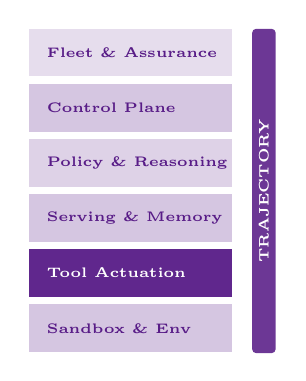
\begin{tikzpicture}
  \protorungsm{3.50}{0.62}{Fleet \& Assurance}{15}{amethyst}
  \protorungsm{2.80}{0.62}{Control Plane}{25}{amethyst}
  \protorungsm{2.10}{0.62}{Policy \& Reasoning}{20}{amethyst}
  \protorungsm{1.40}{0.62}{Serving \& Memory}{25}{amethyst}
  \protorungsm{0.70}{0.62}{Tool Actuation}{95}{amethyst}
  \protorungsm{0.00}{0.62}{Sandbox \& Env}{25}{amethyst}
  \protospine{0.00}{4.12}{TRAJECTORY}{88}{amethyst}
\end{tikzpicture}\\[3mm]
\protocap{A. Current (ships today)}{Six rungs plus the TRAJECTORY spine. Already correct; nothing forces a change.}
\end{minipage}\hfill
% ---------- B: + cadence/scope column ----------
\begin{minipage}[t]{3.4cm}
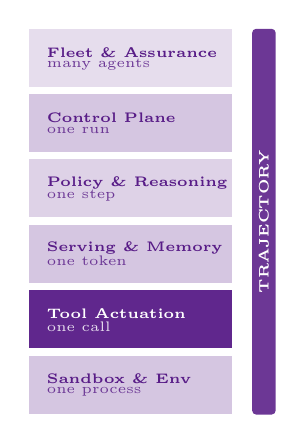
\begin{tikzpicture}
  \protorungsmrt{3.85}{0.75}{Fleet \& Assurance}{many agents}{15}{amethyst}
  \protorungsmrt{3.02}{0.75}{Control Plane}{one run}{25}{amethyst}
  \protorungsmrt{2.19}{0.75}{Policy \& Reasoning}{one step}{20}{amethyst}
  \protorungsmrt{1.36}{0.75}{Serving \& Memory}{one token}{25}{amethyst}
  \protorungsmrt{0.53}{0.75}{Tool Actuation}{one call}{95}{amethyst}
  \protorungsmrt{-0.30}{0.75}{Sandbox \& Env}{one process}{25}{amethyst}
  \protospine{-0.30}{4.60}{TRAJECTORY}{88}{amethyst}
\end{tikzpicture}\\[3mm]
\protocap{B. + unit-of-work column}{Each rung names the unit it reasons about. vol4's cadence column, ported to a stack with no clock.}
\end{minipage}\hfill
% ---------- C: + part gutter ----------
\begin{minipage}[t]{3.6cm}
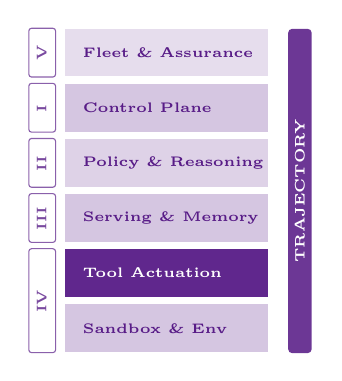
\begin{tikzpicture}
  \foreach \y/\h/\n in {3.50/0.62/V, 2.80/0.62/I, 2.10/0.62/II, 1.40/0.62/III, 0.00/1.32/IV} {
    \node[draw=amethyst!70,line width=0.4pt,rounded corners=1pt,
          minimum width=0.34cm,minimum height=\h cm,anchor=south west,inner sep=0pt]
          at (-0.45,\y) {};
    \node[rotate=90,text=amethyst,opacity=0.8,
          font=\rmfamily\fontsize{4.4}{5}\selectfont\bfseries] at (-0.28,\y+\h/2) {\n};
  }
  \protorungsm{3.50}{0.62}{Fleet \& Assurance}{15}{amethyst}
  \protorungsm{2.80}{0.62}{Control Plane}{25}{amethyst}
  \protorungsm{2.10}{0.62}{Policy \& Reasoning}{20}{amethyst}
  \protorungsm{1.40}{0.62}{Serving \& Memory}{25}{amethyst}
  \protorungsm{0.70}{0.62}{Tool Actuation}{95}{amethyst}
  \protorungsm{0.00}{0.62}{Sandbox \& Env}{25}{amethyst}
  \protospine{0.00}{4.12}{TRAJECTORY}{88}{amethyst}
\end{tikzpicture}\\[3mm]
\protocap{C. + part gutter}{vol2 does this, but its rungs are 10\,mm. At vol3's 6.2\,mm only a bare numeral fits, so the gutter stops reading as ``Part''.}
\end{minipage}\hfill
\begin{minipage}[t]{4.6cm}\raggedright
\textbf{\footnotesize What vol3 is actually missing}\\[2pt]
{\fontsize{7}{9}\selectfont
Not a redesign. vol1 and vol2 each define a \texttt{\dots stackfull} variant and use it on
the About page with three sample chapters, so the reader meets the stack before the
chapters do. vol3 defines no full variant and its About page never shows the stack.
vol4 has the same gap.\\[4pt]
Recommendation: keep A, add the missing full variant.}
\end{minipage}
\end{document}
